\documentclass{article}

\usepackage[utf8]{inputenc}

\usepackage{amsmath}
\usepackage{graphicx}
\usepackage{amssymb}
\usepackage{float}
\usepackage{listings}
\usepackage{hyperref}

\setlength{\parskip}{\baselineskip}%
\setlength{\parindent}{0pt}%

\begin{document}

\title{Drone Project}
\author{Pender L.}
\date{January 2023}
\maketitle


\section{Introduction}

Building a drone from scratch allows for greater flexibility in terms of hardware selection, sensor integration, and firmware development. This report focuses on the state estimation and control system design for a custom-built drone designed to operate in harsh environments. The challenges and opportunities associated with developing both the hardware and firmware components are highlighted, with a particular emphasis on the drone's ability to withstand extreme conditions.

State estimation plays a vital role in the drone's navigation system, enabling accurate determination of the vehicle's position, velocity, and orientation, even in challenging environments. By fusing data from various sensors, such as inertial measurement units (IMUs), GPS, and vision-based sensors, the state estimation algorithm can provide a reliable estimate of the drone's state vector. However, the integration of multiple sensors and the development of robust estimation algorithms require careful consideration of sensor characteristics, noise properties, and computational constraints, especially when operating in harsh conditions.

The control system design is another critical aspect of a custom-built drone for harsh environments. It involves the development of algorithms that generate appropriate control inputs to the propulsion system based on the estimated state and desired trajectory. The control system must be robust enough to handle disturbances and uncertainties associated with extreme environmental factors.

This report covers the theory and practical aspects of state estimation and control system design for a custom-built drone designed for harsh environments. It covers topics such as sensor fusion, stochastic and deterministic error modeling, nonlinear control techniques, and firmware architecture.


% Aims, Objectives and context
\section{Theory}

\subsection{State Estimation}

The state estimation process and error models are based heavily on the guide by Jay A. Farrell et. al. \cite{error_modelling}.

The navigation system propagates the vehicle's
state vector through time by integrating the nonlinear
model of $\dot{\hat{\mathbf{x}}} = f(\hat{\mathbf{x}}, \hat{\mathbf{u}})$, an error denoted by $\delta\mathbf{x}_v = \mathbf{x} - \hat{\mathbf{x}}$ will
develop between the actual and estimated state vectors.
The error states then contain an position, velocity, and this augmented error state to give 9 states in total.
This vehicle state error vector can
be estimated in real time using measurements from the
aiding sensors.
The estimation algorithm incorporates a linearized state-space model for
the error state
\begin{equation}
    \delta \dot{\mathbf{x}}_v(t) =  \mathbf{F}(t) \delta \mathbf{x}_v(t) + \mathbf{G} \delta \mathbf{u}(t)
\end{equation}
Where $\mathbf{F}(t)$ is the Jacobian of the nonlinear model $f(\hat{\mathbf{x}}, \hat{\mathbf{u}})$, and $\mathbf{G}$ is the Jacobian of the input vector $\hat{\mathbf{u}}$.
The error in the input vector is given by $\delta\mathbf{u} = \mathbf{u} - \hat{\mathbf{u}}$

The real-time state estimation process is designed to
estimate the augmented state vector
\begin{equation}
    \mathbf{x} = \begin{bmatrix}
        \delta \mathbf{x}_v(t) \\
        \mathbf{x}_d(t) \\
        \mathbf{x}_z(t)
    \end{bmatrix}
\end{equation}

Where the state vectors $\mathbf{x}_d(t)$ and $\mathbf{x}_z(t)$ are augmented state vectors for deterministic and stochastic disturbances respectively.

The measured signal $\hat{\mathbf{u}}(t)$ differs from desired signal $\mathbf{u}(t)$ from deterministic and stochastic.
\begin{equation}
    \hat{\mathbf{u}}(t) = \mathbf{u}(t) + \mathbf{d}(\mathbf{u}(t)) + \mathbf{z}(t)    
\end{equation}

\subsubsection{Stochastic Error Modelling}

\begin{align}
    \dot{\mathbf{x}_z} &= \mathbf{A}_z \mathbf{x}_z(t) + \mathbf{B}_z \boldsymbol{\omega}_z(t) \\
    \mathbf{z}(t) &= \mathbf{C}_z \mathbf{x}_z(t) + \boldsymbol{\eta}_z(t)
\end{align}
where $\mathbf{A}_z \in \mathbb{R}^{n_z \times n_z}$, $\mathbf{B}_z \in \mathbb{R}^{n_z \times p}$, $\mathbf{C}_z \in \mathbb{R}^{3 \times n_z}$, and $n_z$ is the number of states in the stochastic error model.
The parameter p represents the number of distinct and independent noise processes in the differential equation portion
of the IMU error model.
The random signals $\boldsymbol{\omega}_z(t)$ and $\boldsymbol{\eta}_z(t)$ are mutually independent Gaussian white-noise processes with power spectral densities (PSDs)
$\mathbf{S}_{\boldsymbol{\omega}_z}(\omega) \in \mathbb{R}^{p \times p}$ and $\mathbf{S}_{\boldsymbol{\eta}_z}(\omega) \in \mathbb{R}^{3}$, respectively.

The corresponding frequency domain representation is given by
\begin{equation}
    \mathbf{Z}(s) = \mathbf{T}(s)\boldsymbol{\Omega}_z(s) + \boldsymbol{\eta}_z(s)
\end{equation}
Where the transfer function $\mathbf{T}(s)$ is given by
\begin{equation}
    \mathbf{T}(s) = \mathbf{C}_z (s\mathbf{I} - \mathbf{A}_z)^{-1} \mathbf{B}_z
\end{equation}
Then the power spectral density of the stochastic error is given by
\begin{equation}
    \mathbf{S}_{z} = \mathbf{T}(j\omega) \mathbf{S}_{\boldsymbol{\omega}_z} \mathbf{T}^T(-j\omega) + \mathbf{S}_{\boldsymbol{\eta}_z}
\end{equation}
Assuming that all elements of the driving noise vector
$\boldsymbol{\omega}_z(t)$ and the output noise $\boldsymbol{\eta}_z(t)$ are mutually independent
and white, this simplifies to

\begin{equation}
    \mathbf{S}_{z} = \sum_{i=1}^{p} \mathbf{T}_i(j\omega) \mathbf{S}_{\boldsymbol{\omega}_zi} \mathbf{T}_i^T(-j\omega) + \mathbf{S}_{\boldsymbol{\eta}_z}
\end{equation}
Where $\mathbf{T}_i(s)$ is the 3 axes transfer functions from the ith
component of $\boldsymbol{\omega}_z$ to $\mathbf{z}(t)$, and $\mathbf{B}_z \in \mathbb{R}^{n_z \times 3}$ is the ith column of $\mathbf{B}_z$.


\subsubsection{Deterministic Error Modelling}


\subsection{Control System Design}

The measured states of the drone are given as follows
\begin{equation}
    \mathbf{x} = \begin{bmatrix} \mathbf{r}_p \\ \boldsymbol{\alpha} \\ \mathbf{\dot{r}}_p \\  \boldsymbol{\omega}  \end{bmatrix}, \quad \mathbf{u} = \begin{bmatrix} \Omega_1^2 \\ \Omega_2^2 \\ \Omega_3^2 \\ \Omega_4^2 \end{bmatrix}
\end{equation}

\begin{align}
    \mathbf{\dot{x}} &= \mathbf{Ax} + \mathbf{Bu} \\
    \mathbf{y} &= \mathbf{Cx} + \mathbf{Du}
\end{align}

The drone transfer function is therefor given by
\begin{equation}
    \mathbf{G} = \mathbf{C} (s\mathbf{I} - \mathbf{A})^{-1} \mathbf{B} + \mathbf{D}
\end{equation}
The goal is to find a controller matrix K which gives the overall transfer function
\begin{equation}
    \mathbf{G}_{cl} = \mathbf{C} (s\mathbf{I} - \mathbf{A} + \mathbf{BK})^{-1} \mathbf{B} + \mathbf{D}
\end{equation}


The nonlinear state space model is given by
\begin{equation}
    \mathbf{\dot{x}} = \begin{bmatrix}
        \mathbf{\dot{r}}_p \\
        \boldsymbol{\omega} \\
        \mathbf{\dot{r}}_p \\
        \boldsymbol{\dot{\omega}}
    \end{bmatrix} = \begin{bmatrix}
        \mathbf{x}_1 \\
        \mathbf{x}_2 \\
        \mathbf{R}(\mathbf{f}_p + \mathbf{f}_b) / m - \mathbf{g} \\
        \mathbf{I}^{-1} (\boldsymbol{\tau}_p - \boldsymbol{\omega} \times \mathbf{I} \boldsymbol{\omega})
    \end{bmatrix}
\end{equation}
Where row 3 and 4 are the translational and rotational dynamics respectively.

Where $\mathbf{R}$ is the rotation matrix from the body frame to the inertial frame,
$\mathbf{f}_p$, $\boldsymbol{\tau}$ is the respective force and torque from the propellers in the body frame,
\begin{equation}
    \mathbf{f}_p = \sum{\mathbf{f}_i}
\end{equation}
\begin{equation}
    \boldsymbol{\tau}_p = \sum{\boldsymbol{\tau}_i + \mathbf{r}_{Pi} \times (\mathbf{f}_i)}
\end{equation}
Where $\boldsymbol{\tau}_i$ is the torque from the $i$th propeller, and $\mathbf{r}_{Pi}$ is the position of the $i$th propeller from the center of mass.
The drag body force is given by $\mathbf{f}_b$ is defined as follows:
\begin{equation}
    \mathbf{f}_b = -\frac{1}{2} C_D \rho (\mathbf{A}_r \mathbf{v}_r ) \mathbf{v}_r
\end{equation}
Where $\mathbf{v}_r$ is the velocity of the drone relative to the air, and $\rho$ is the air density.
For a wind speed $\mathbf{v}_w$, the relative velocity is given by
\begin{equation}
    \mathbf{v}_r = \mathbf{\dot{r}}_p - \mathbf{v}_w
\end{equation}


\subsubsection{LQR Designed Controller}

The cost function associated with optimal control is defined as follows:

\begin{equation}
  J = \int_0^\infty \left( \mathbf{x}^T \mathbf{Q} \mathbf{x} + \mathbf{u}^T \mathbf{R} \mathbf{u} \right) dt
\end{equation}

Where the matricies $\mathbf{Q}$ and $\mathbf{R}$ are the diagonal state and control weighting matricies respectively.
They are chosen using Bryson's rule, a heuristic method for choosing the matricies shown below \cite{feedback_control_of_dynamic_systems}

\begin{equation}
  \mathbf{Q}_{ii} = \frac{1}{\text{max}(\mathbf{x}_i)^2} \quad \mathbf{R} = \frac{1}{\text{max}(u)^2}
\end{equation}

Where max is an approximation for the maximum desired value of the state or control input.
From this the closed loop response can be tuned to have desired characteristics, such as fast response or minimal control effort.
The result of LQR is the gain matrix $\mathbf{K}$ such that $\mathbf{u} = -\mathbf{Kx}$ that minimises the cost function.

\section{Design}

\subsection{Purchased Parts}

\begin{table}[H]
    \centering
    \begin{tabular}{|l|r|}
        \hline
        Component & Price \\
        \hline
        BMP280 & £6.00 \\
        BNO055 & £27.59 \\
        Pi Pico & £4.00 \\
        BetaFPV diversity reciever & £28.99 \\
        1300 mAh 3s LiPo & £35.99 \\
        Custom PCB & £66.00 \\
        Drone Motors + ESCs & £32.00 \\
        Drone blades & £20.00 \\
        Dyson Center Costs & £20.00 \\
        \hline
    \end{tabular}
    \caption{Purchased Parts}
\end{table}


\subsection{Prototype Development}

\begin{figure}[H]
    \centering
    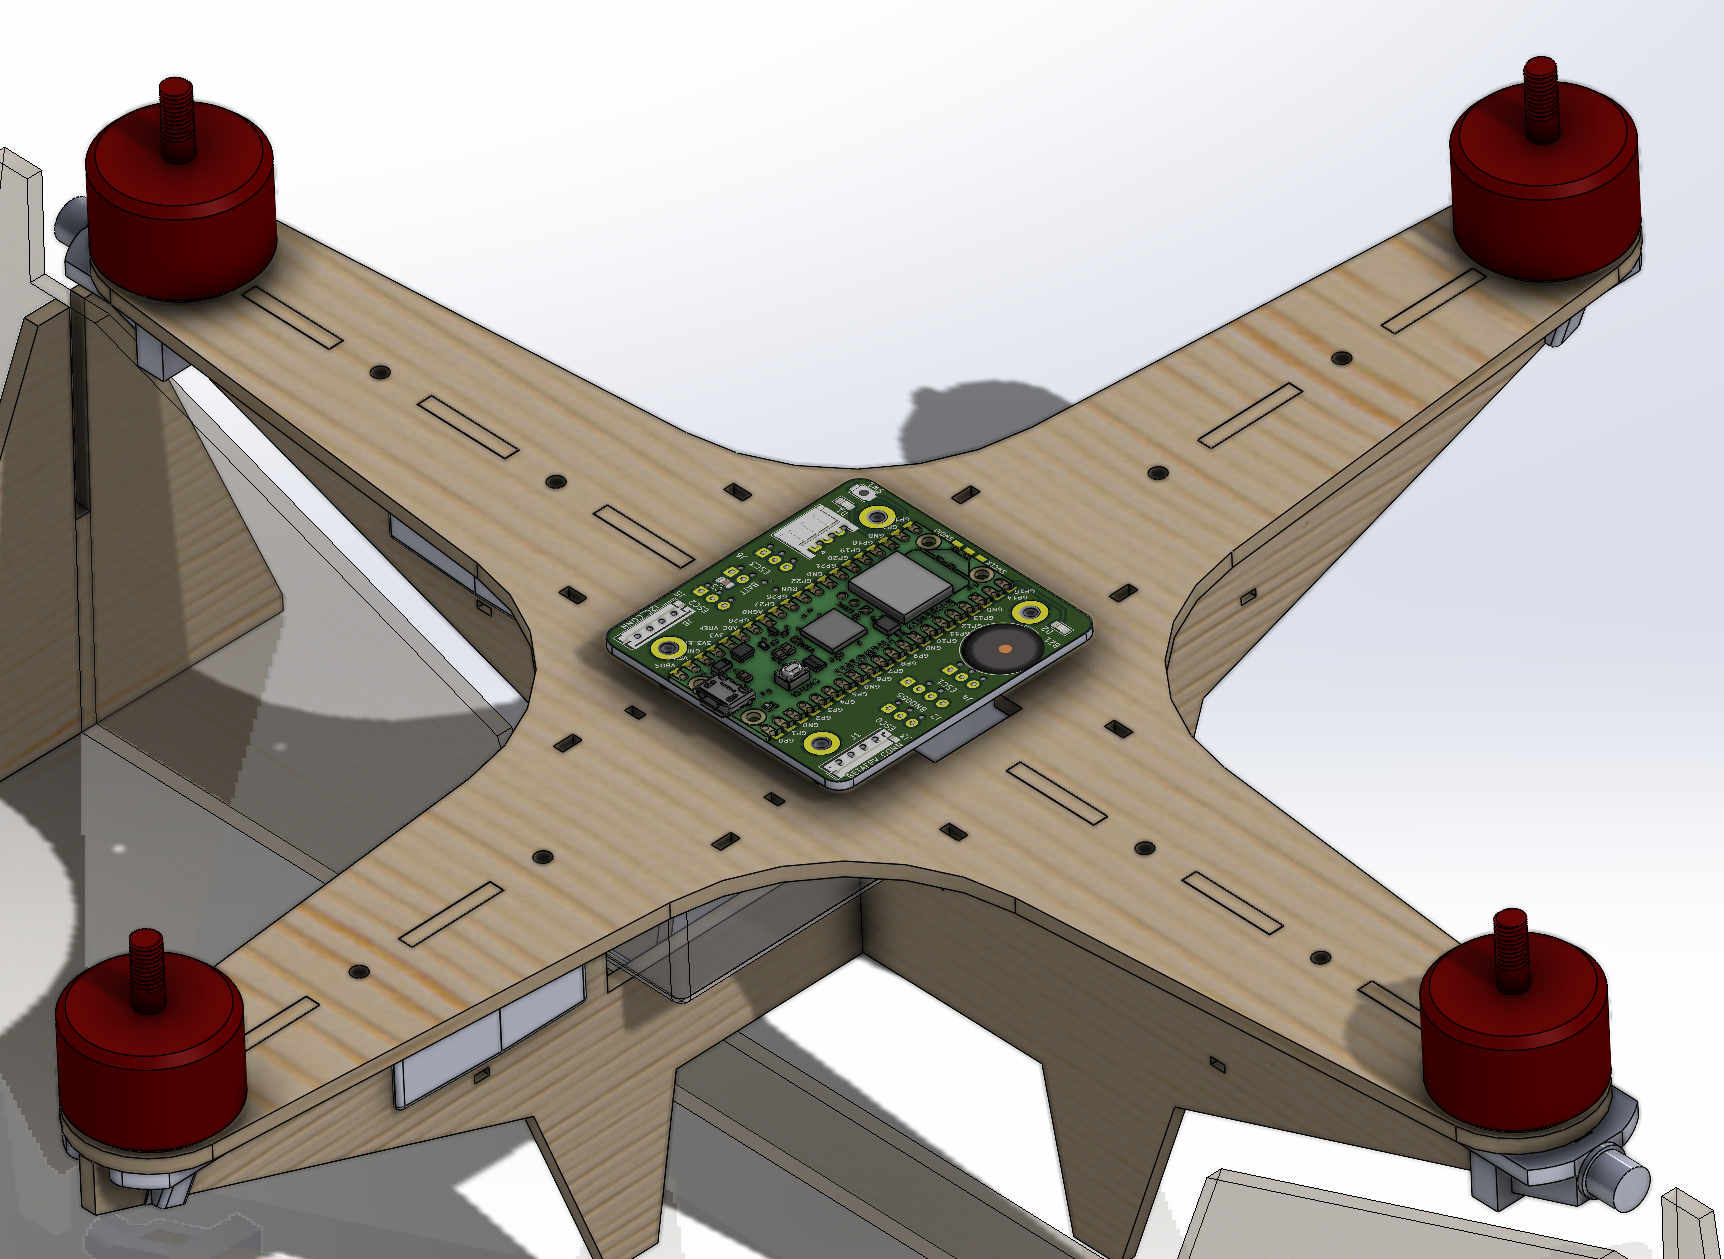
\includegraphics[width=0.8\textwidth]{progress_cad.png}
    \caption{Final CAD Design}
\end{figure}

\begin{figure}[H]
    \centering
    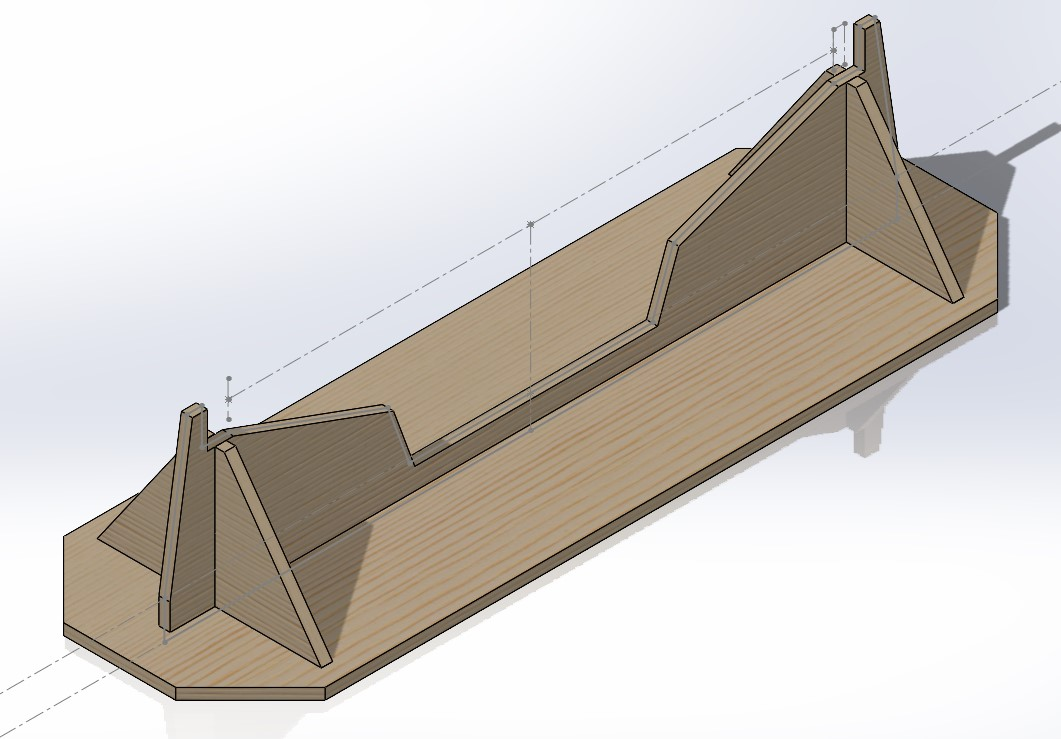
\includegraphics[width=0.8\textwidth]{tuning_stand.jpg}
    \caption{Tuning Stand design}
\end{figure}

\begin{figure}[H]
    \centering
    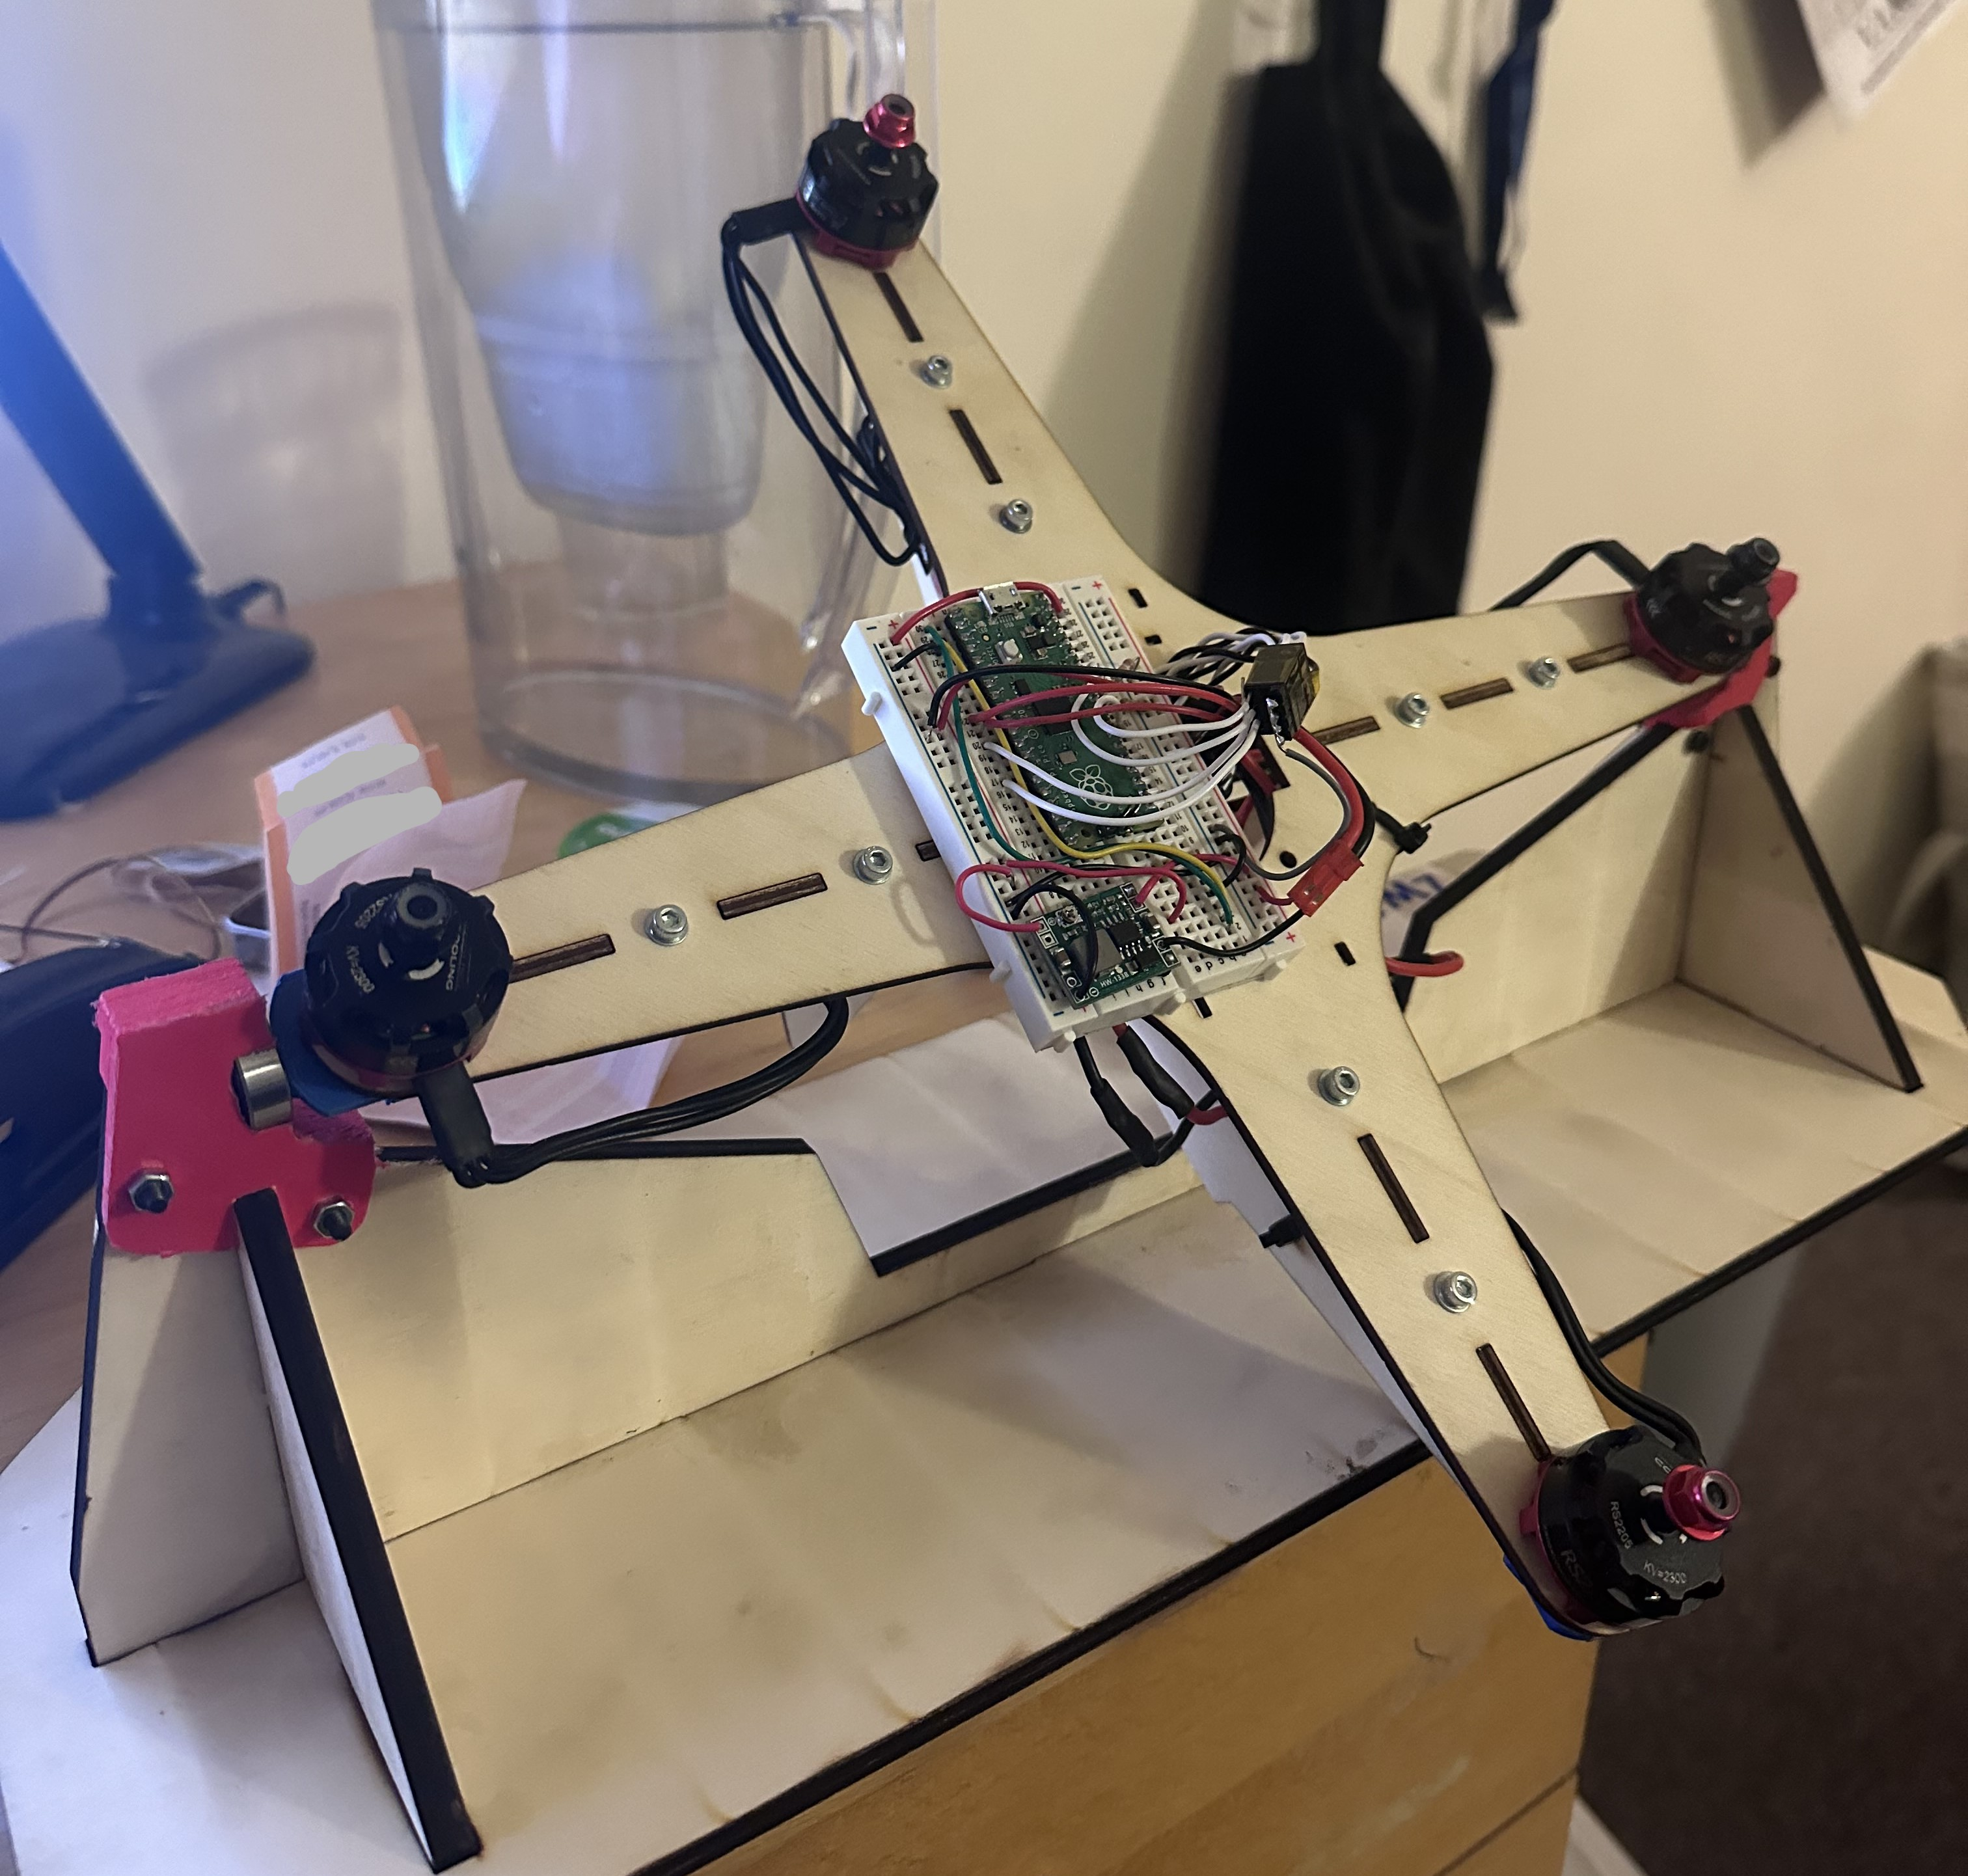
\includegraphics[width=0.8\textwidth]{development.jpg}
    \caption{Prototype Assembly}
\end{figure}

\subsection{PCB Design}

\begin{figure}[H]
    \centering
    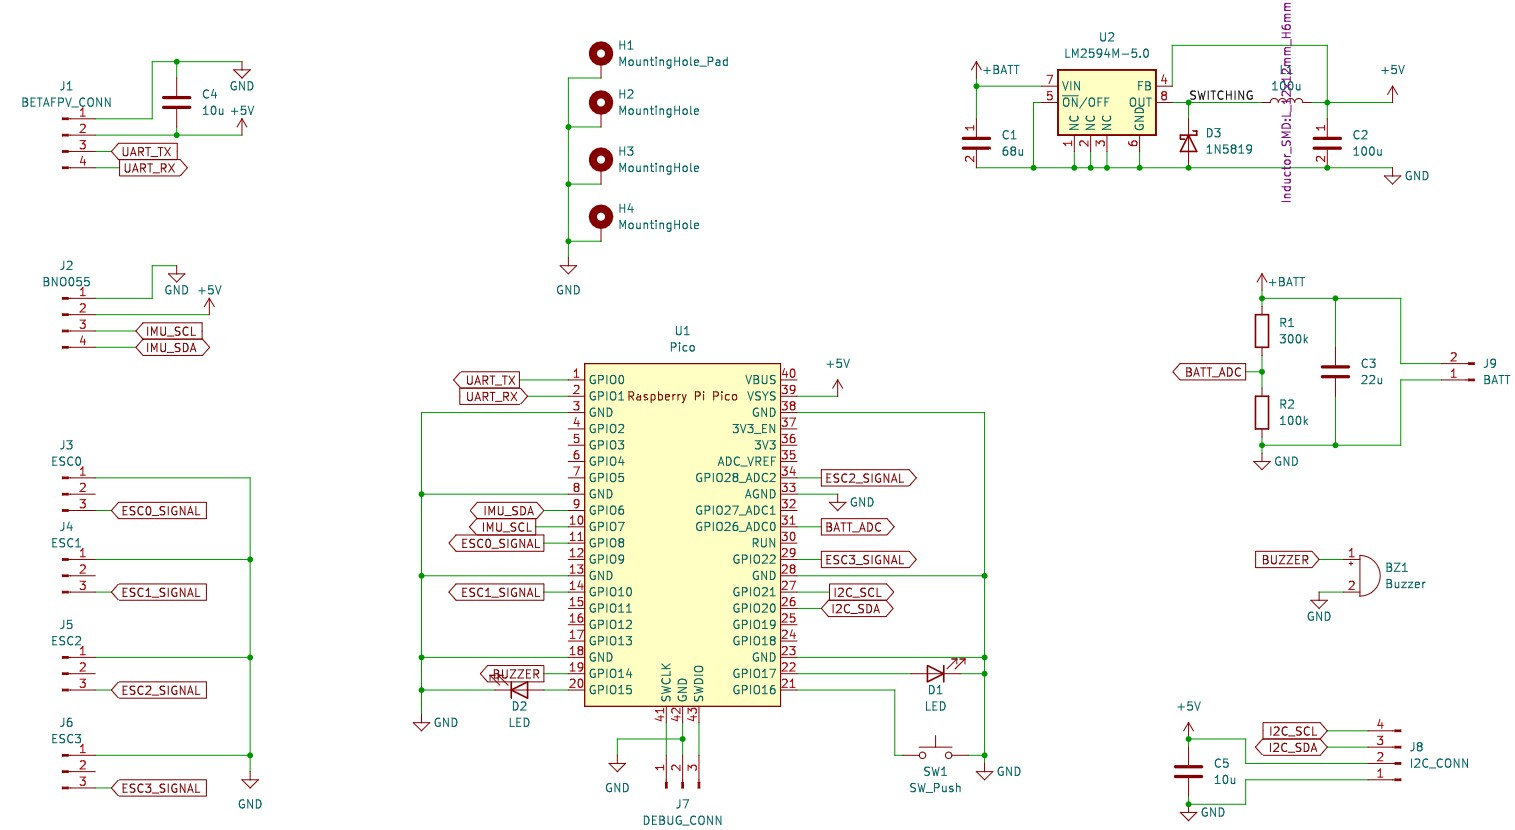
\includegraphics[width=0.8\textwidth]{schematic.jpg}
    \caption{PCB Schematic}
\end{figure}

\begin{figure}[H]
    \centering
    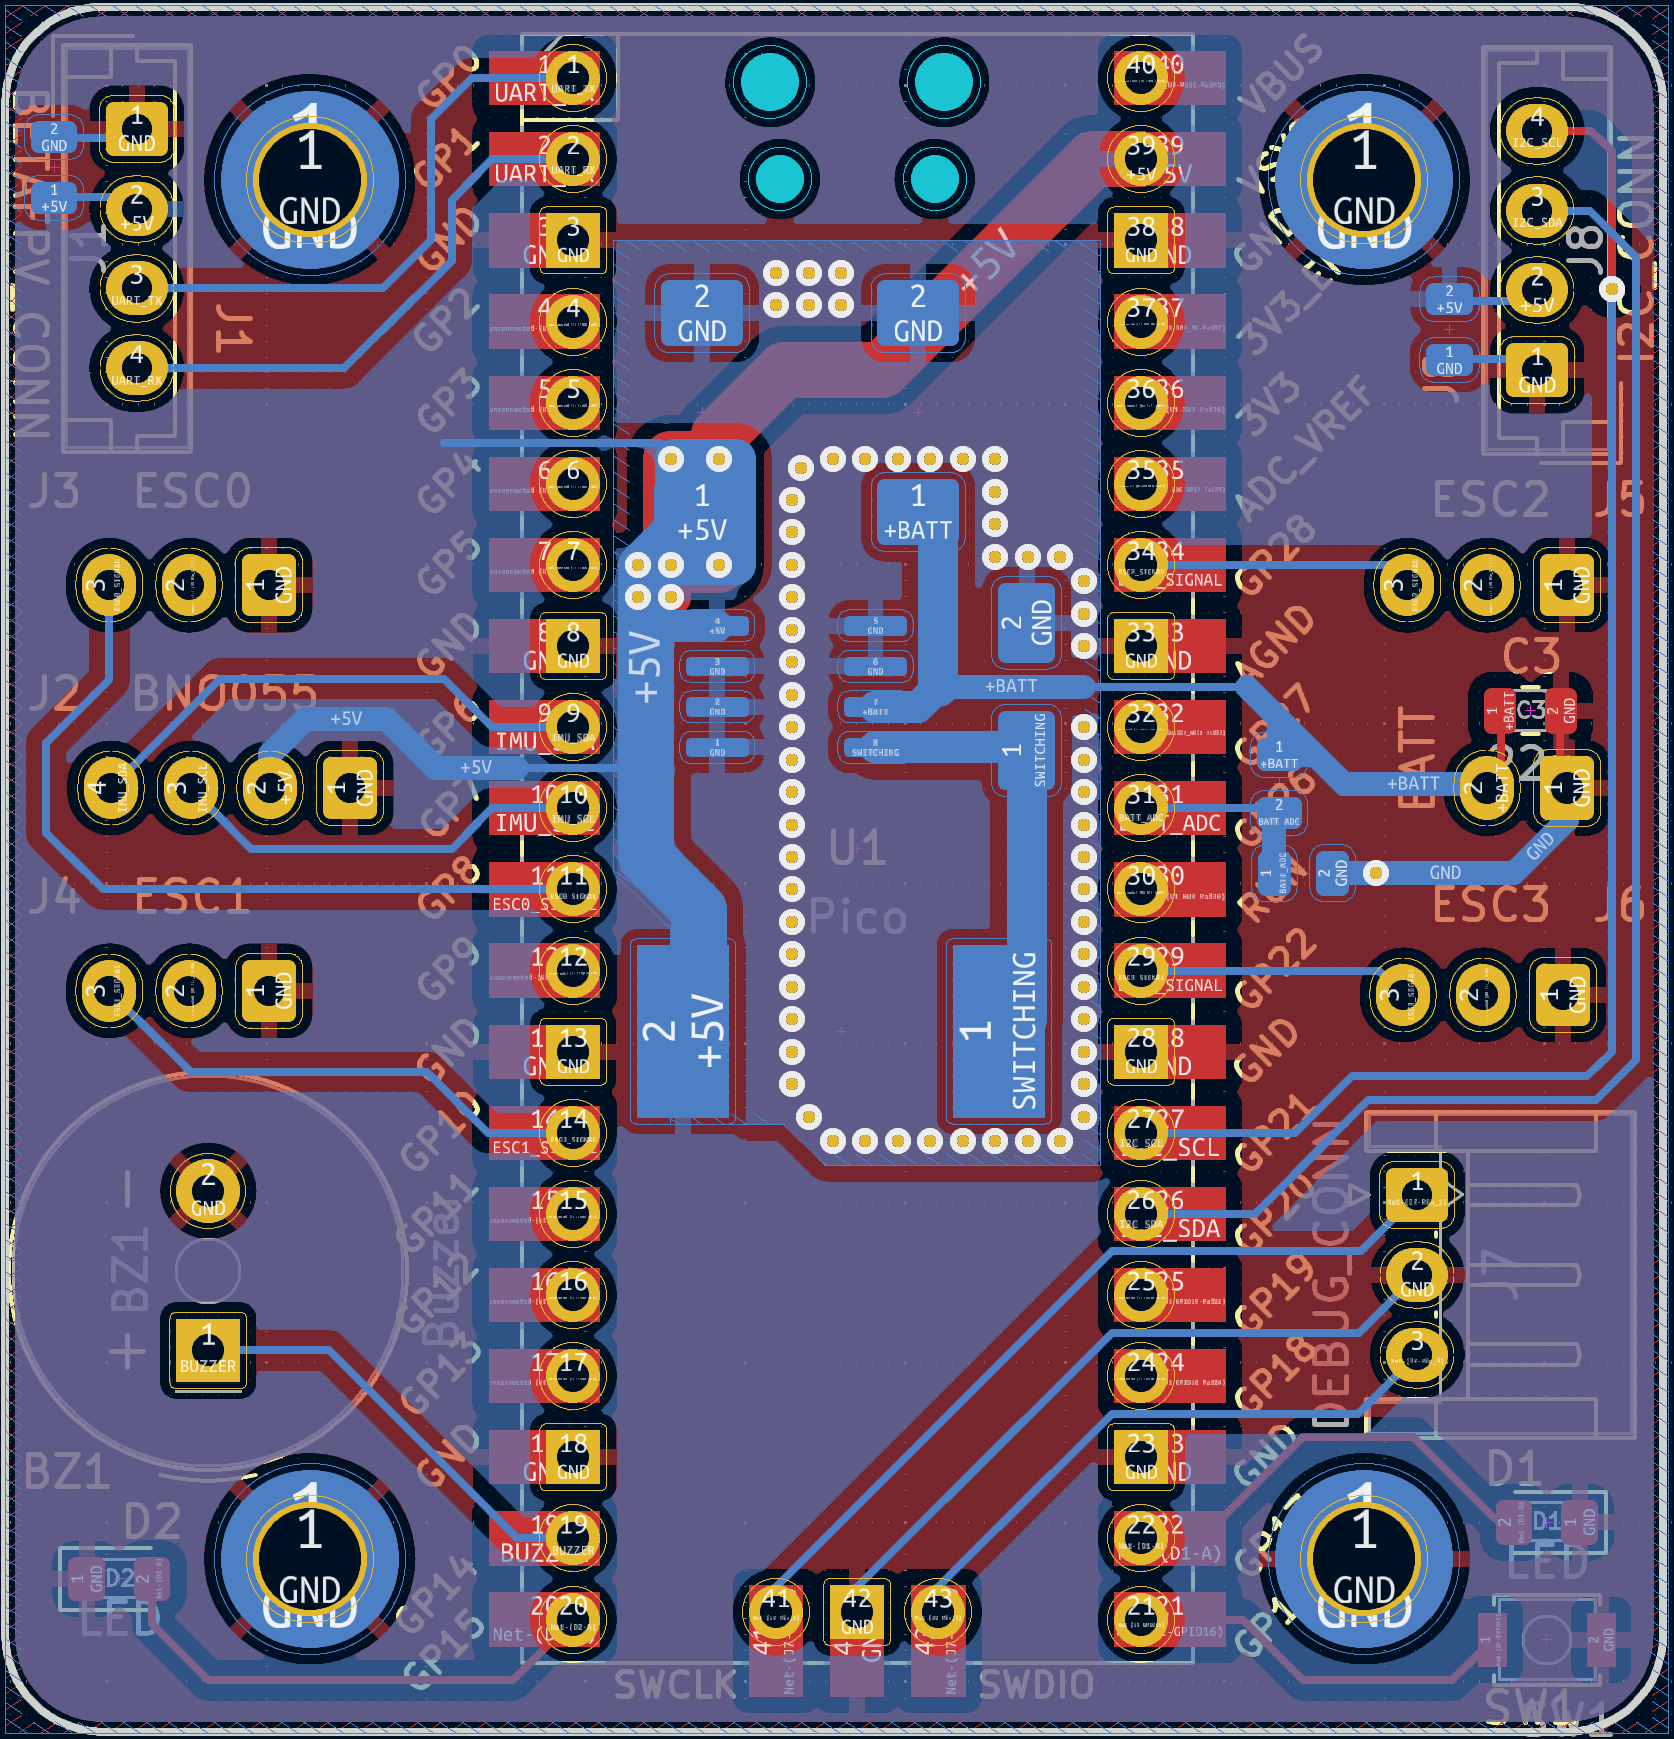
\includegraphics[width=0.8\textwidth]{board_pcb.png}
    \caption{PCB layout}
\end{figure}

\begin{figure}[H]
    \centering
    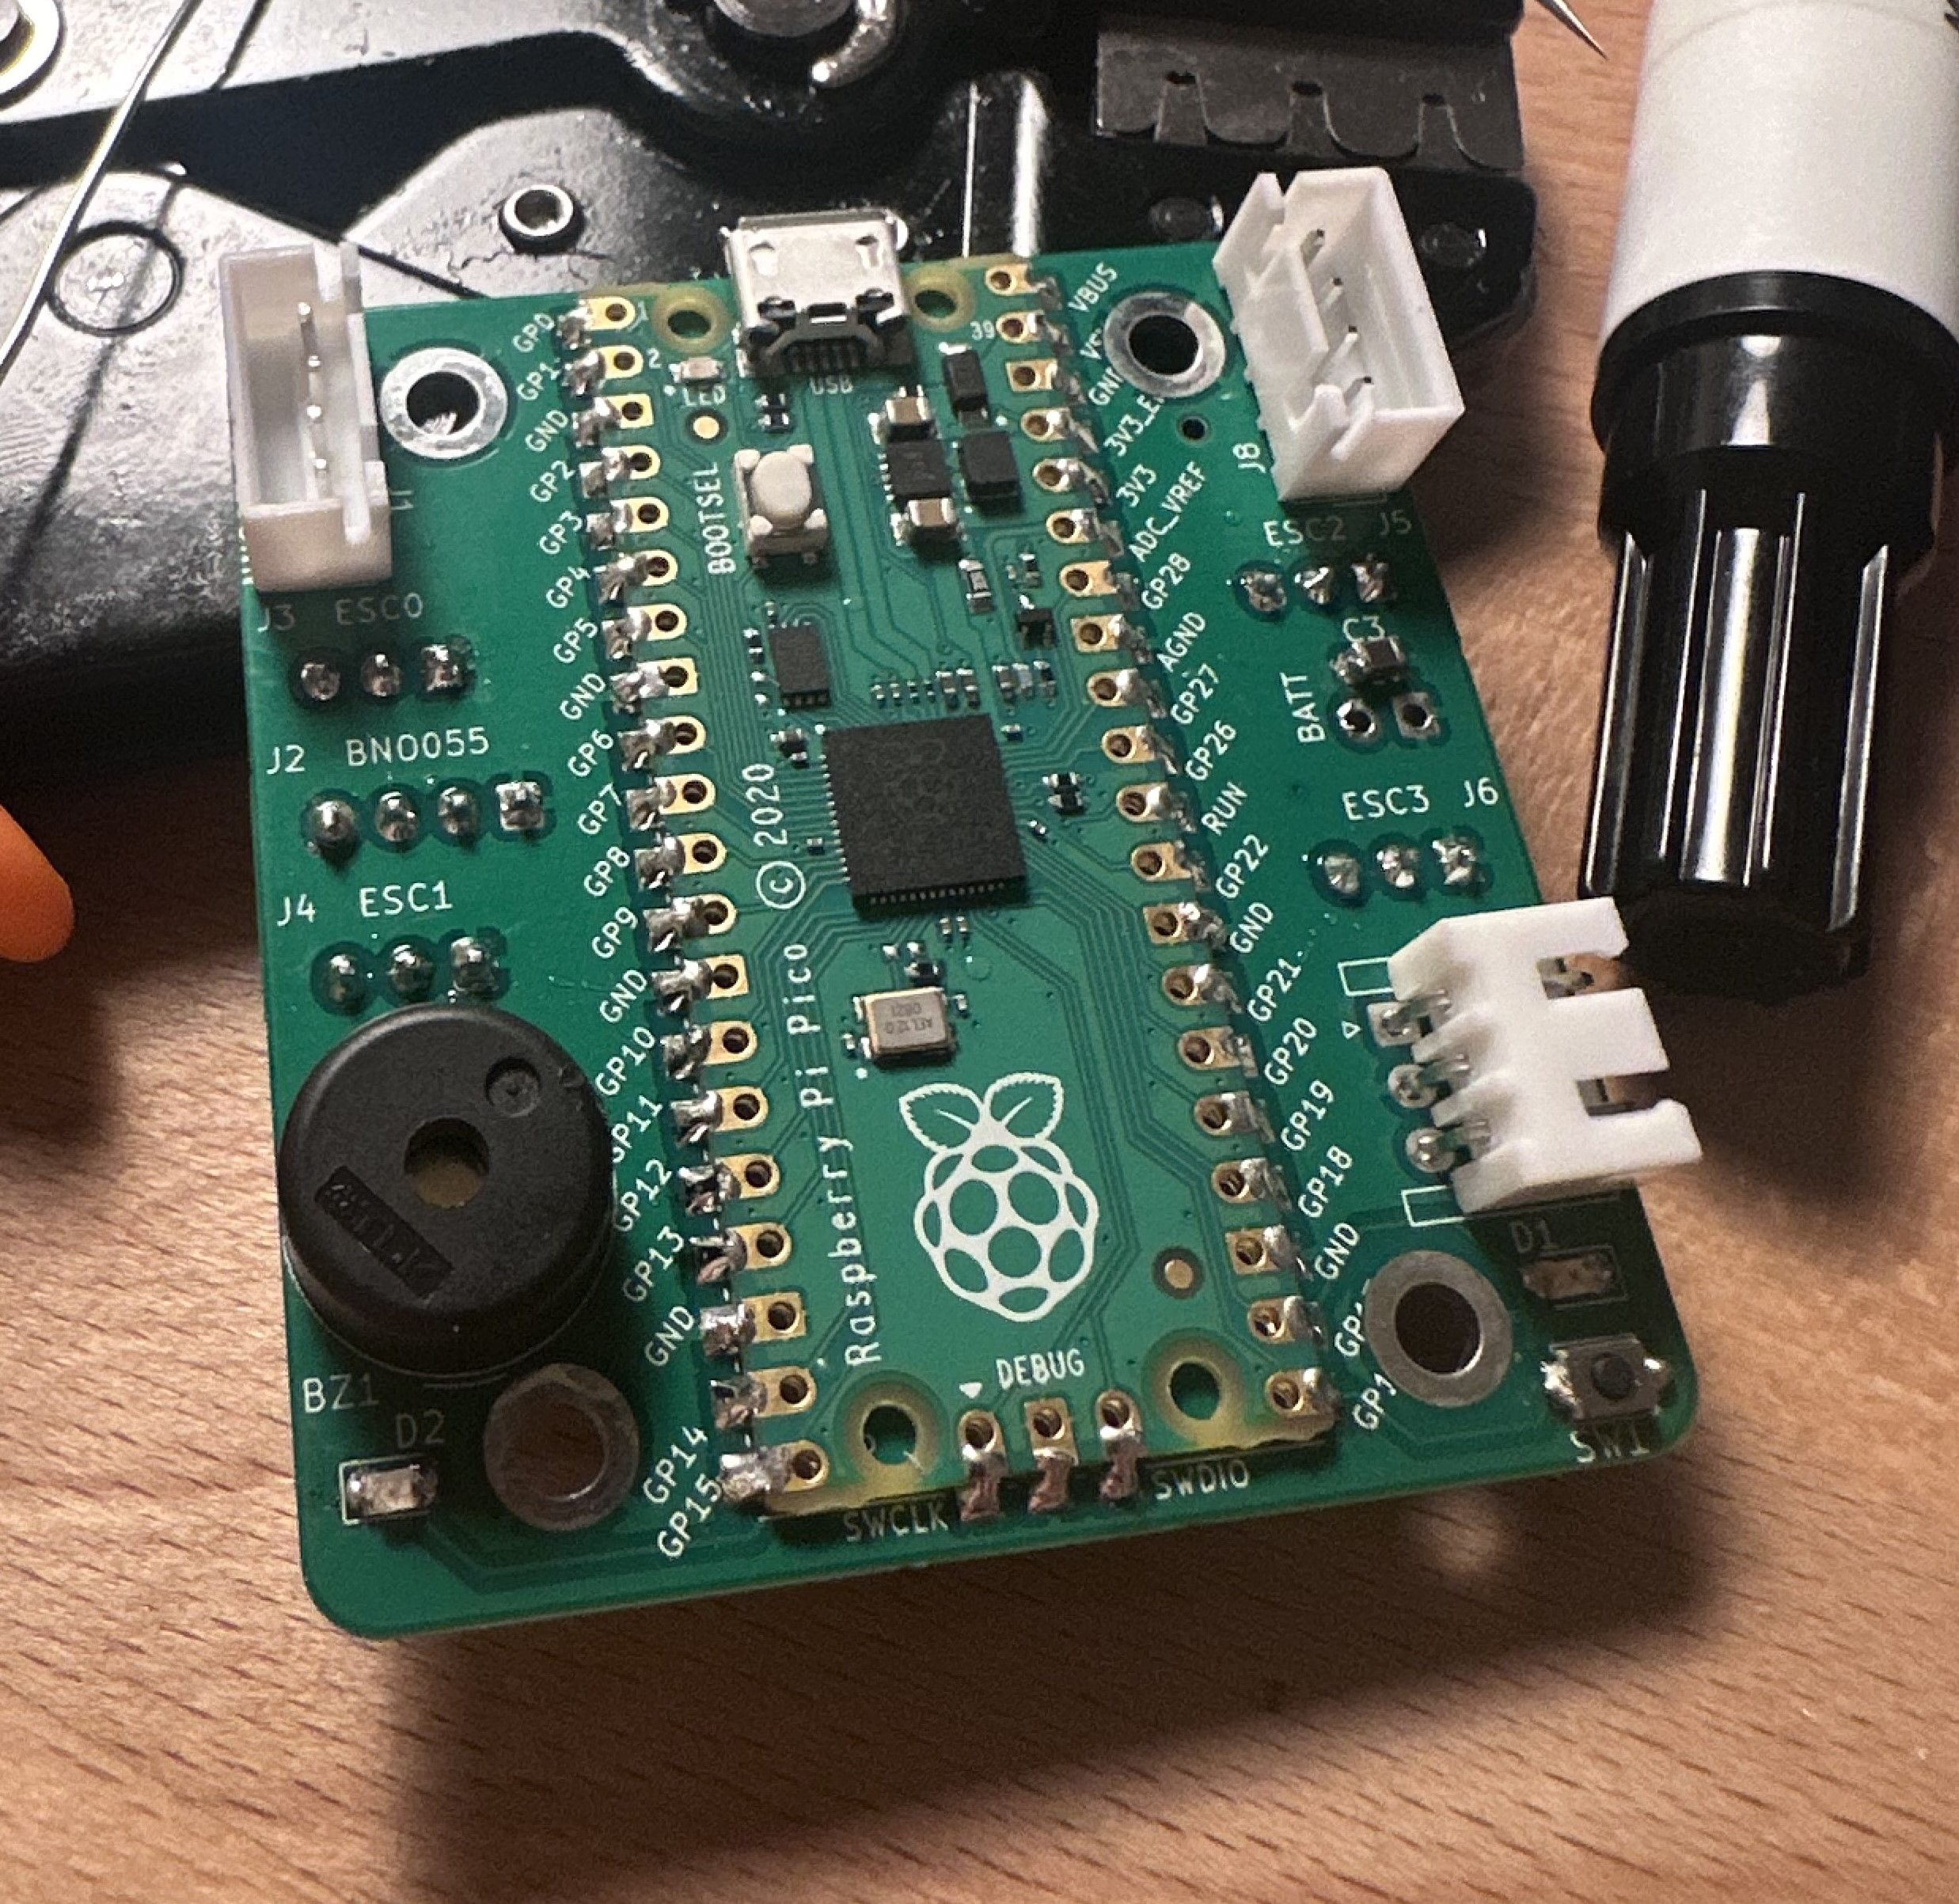
\includegraphics[width=0.8\textwidth]{board_soldered.jpg}
    \caption{Soldered PCB}
\end{figure}


\begin{figure}[H]
    \centering
    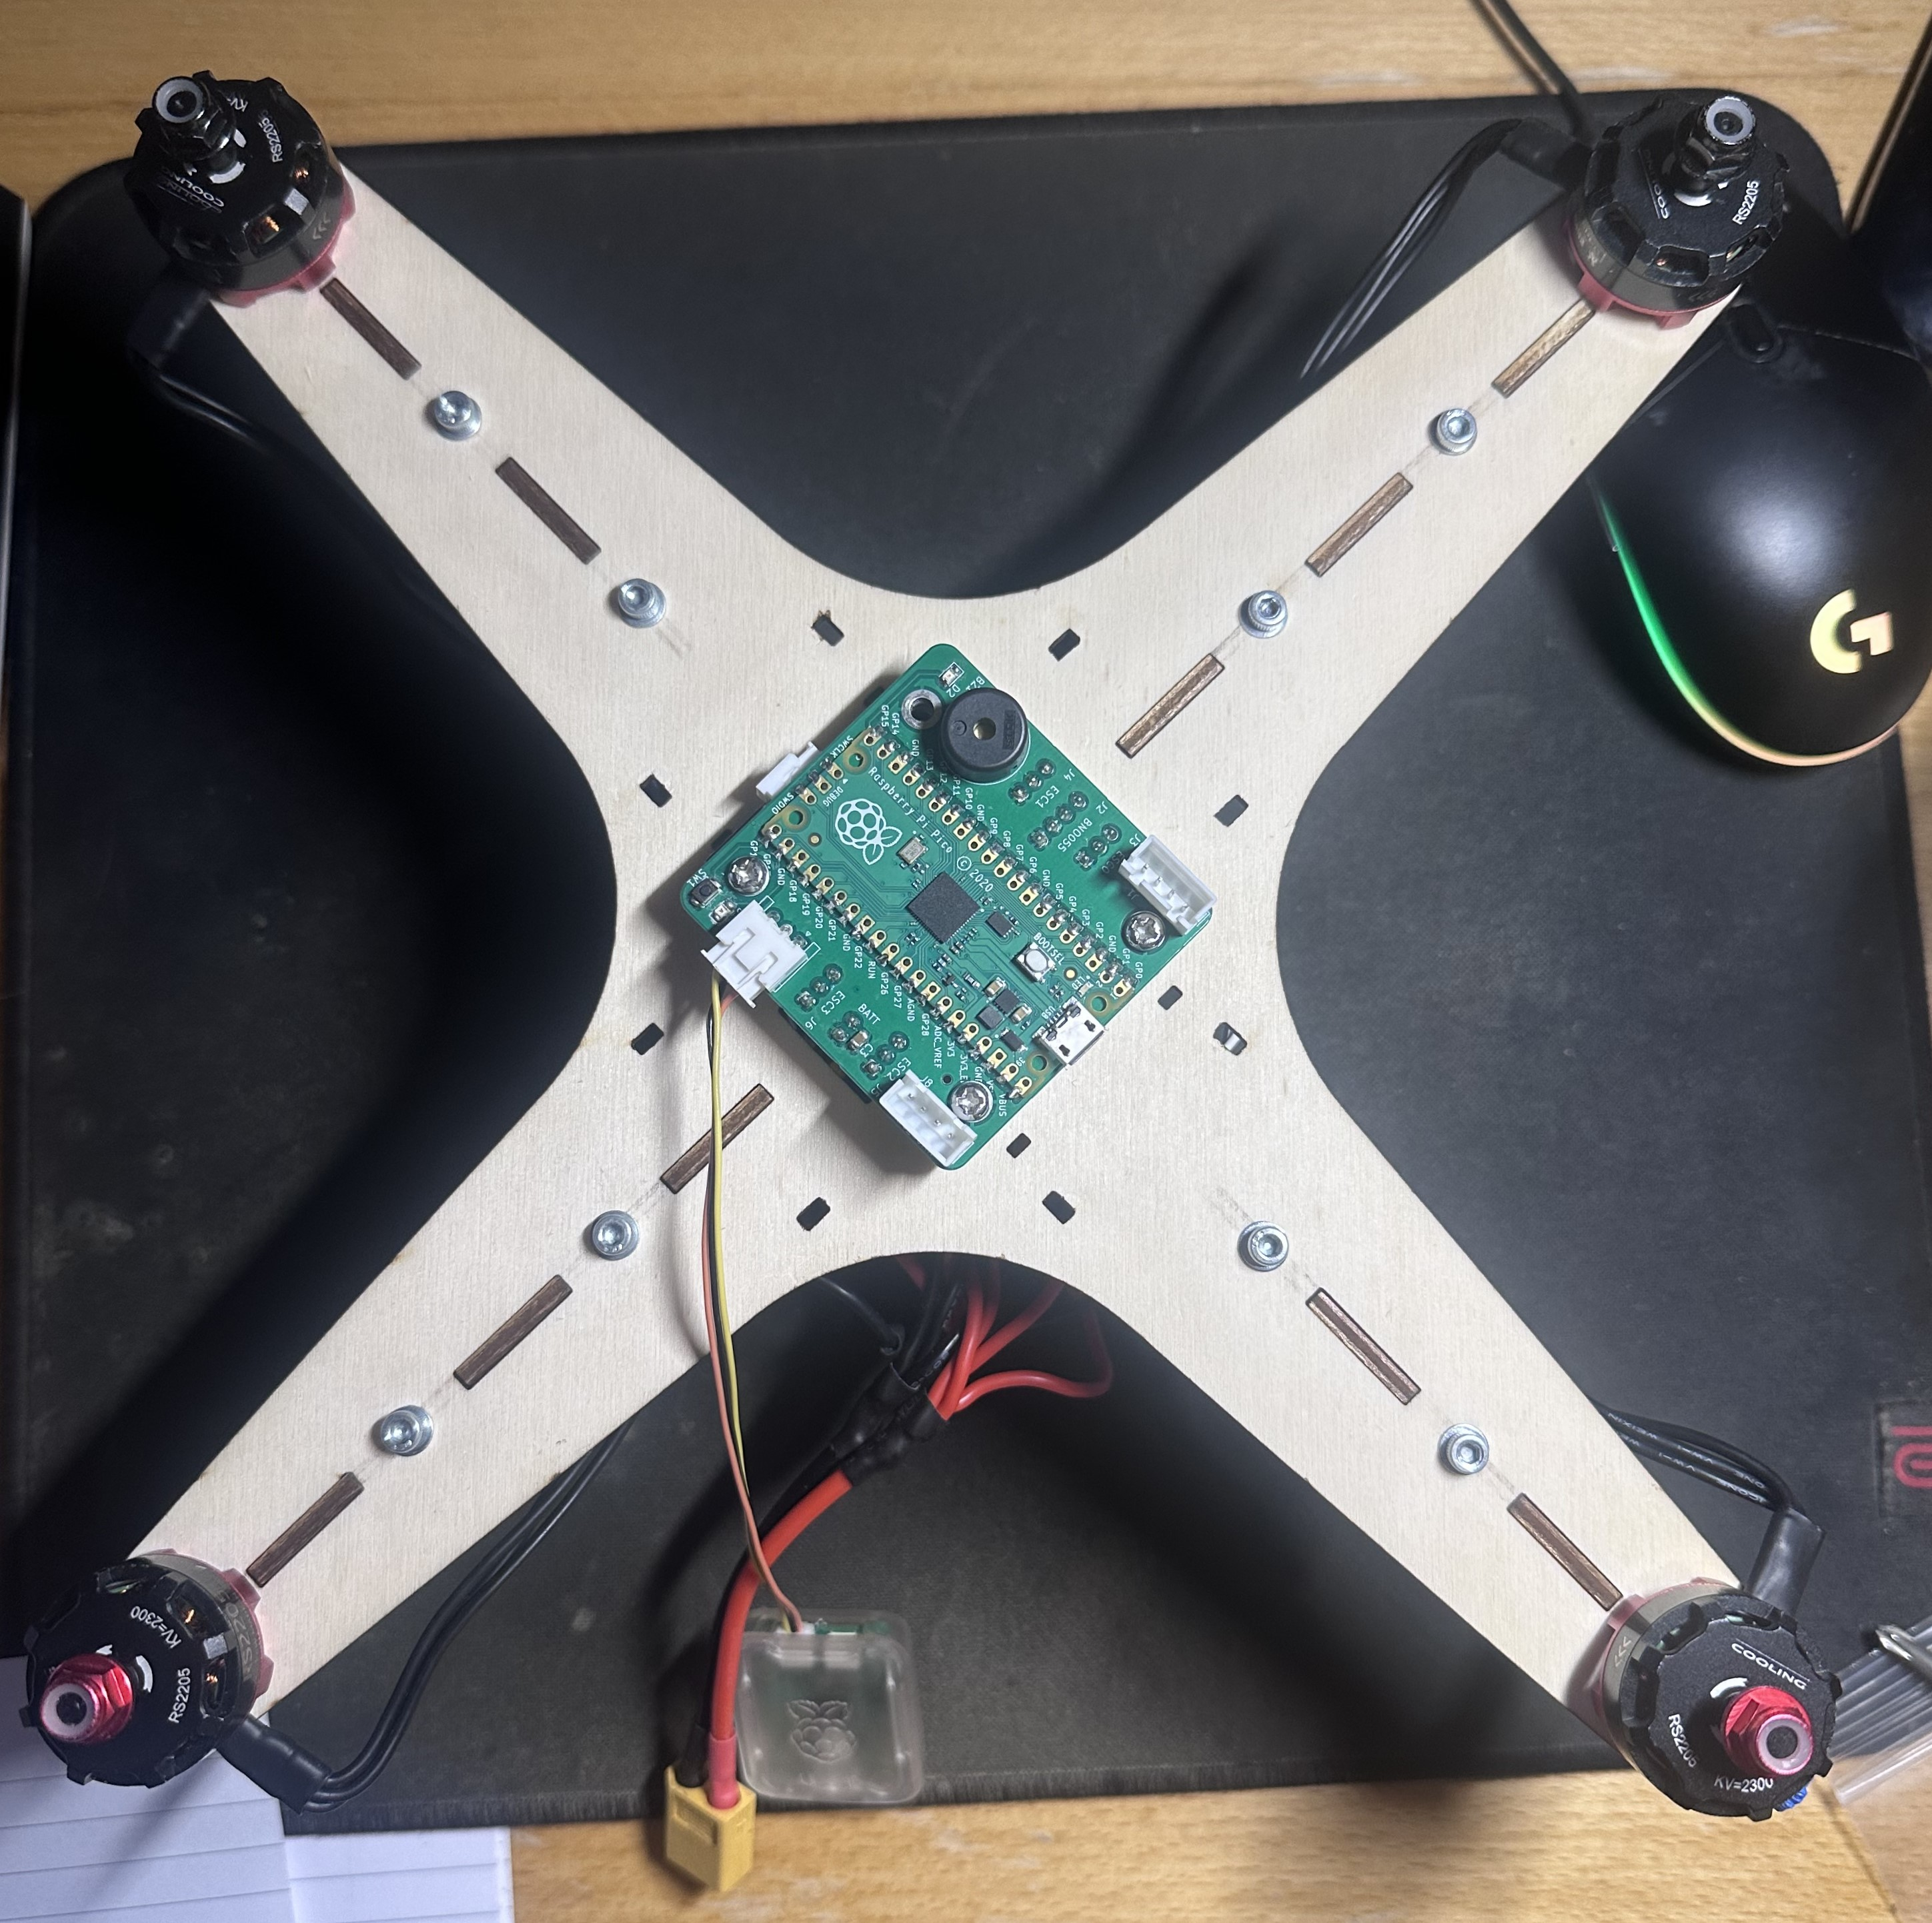
\includegraphics[width=0.8\textwidth]{built.jpg}
    \caption{Drone Assembly}
\end{figure}

\section{Firmware}

The firmware was written in C++, however data collection tools were written in Python and Allan Variance analysis was done in MATLAB using modified code \cite{error_modelling}.

An extended Kalman filter is implemented in observer.cpp, for which tuned allen variance parameters are passed in from the main.cpp file.
Modified libraries were used for the BMP280 and BNO055 sensors, which were interfaced using I2C.

The firmware attempts to make extended use of the Pi Pico's dual core architecture, with the fast radio communications loop running on core 0 and the slower state observer running on core 1.
When a new state estimate is caclulated it is pushed on to the FIFO queue, which is read by the mainloop, for which control will be updated.

\section{Results and future work}

During the course of this project, significant progress was made in the development of the custom-built drone. The hardware components were successfully integrated, including the BMP280 pressure sensor, BNO055 IMU, Pi Pico microcontroller, and the custom PCB. 

However, due to time constraints, the implementation of the state estimation algorithm and the extended Kalman filter was not completed. The firmware development progressed up to the point of sensor interfacing and data collection, but the integration of the state observer and control system remains a crucial step for future work.

Future work will focus on completing the implementation of the state estimation algorithm, integrating the control system, and conducting extensive testing and validation. This will involve refining the firmware, tuning the Kalman filter parameters, and evaluating the drone's performance in various flight scenarios. Additionally, further optimization of the hardware and firmware components may be necessary to achieve the desired flight characteristics and robustness.

\section{Conclusion}

The hardware development of the custom-built drone for harsh environments has been successfully completed, but additional time and effort are required to finalize the state estimation and control system implementation. Future work will focus on programming the extended Kalman filter, integrating control algorithms, and conducting comprehensive testing to ensure reliability and performance in challenging conditions.

Despite the remaining tasks, the progress made in this project lays a solid foundation for the development of drones capable of operating in harsh environments. The insights gained from hardware integration, sensor selection, and firmware development will contribute to the advancement of UAV technology in applications such as search and rescue, environmental monitoring, and industrial inspections.

Future work will involve completing the state estimation and control system implementation and conducting extensive field tests to validate the drone's performance in various harsh environmental scenarios. The custom-built drone for harsh environments represents a significant step forward in the development of UAVs capable of operating in challenging conditions. With the completion of the remaining firmware tasks and rigorous testing, this drone will be a valuable tool for researchers, engineers, and professionals working in fields where drones must navigate extreme environments.

\section{Appendix}


\begin {lstlisting}[language=C++]

#include <stdio.h>
#include "pico/stdlib.h"
#include "hardware/gpio.h"
#include "hardware/i2c.h"
#include "hardware/pwm.h"
#include "hardware/irq.h"
#include "hardware/adc.h"
#include "pico/multicore.h"

#include <Eigen/Dense>
#include "Adafruit_Sensor.h"
#include "Adafruit_BNO055.h"
#include "Adafruit_BMP280.h"
#include "CrsfSerial.h"
#include "motor.h"
#include "observer.h"
#include "control.h"


#include "cal.h"

#define UART_ID uart0
#define BAUD_RATE 420000
#define DATA_BITS 8
#define STOP_BITS 1
#define PARITY    UART_PARITY_NONE
#define UART_TX_PIN 0
#define UART_RX_PIN 1

#define ESC0_PIN 6

#define CALIBRATION_DONE 0xf3
#define DEVICES_FOUND 0xf5
#define BNO055_NOT_FOUND 0xf6
#define BMP280_NOT_FOUND 0xf7
#define VL53L0X_NOT_FOUND 0xf8

CrsfSerial ELRS_rx = CrsfSerial(uart0);

ESC escs[4] = {ESC(8), ESC(10), ESC(28), ESC(22)};

int channel_data;

bool light_flag = false;

int roll_demand;
int pitch_demand;
int yaw_demand;
int throttle;
int input_1;
int input_2;
int input_3;
int input_4;

double roll;
double pitch;
double yaw;

double battery_voltage;


void arm_escs() {
    sleep_ms(500);
    for (int i=0; i<4; i++)
    {
        escs[i].setSpeed(200);
        escs[i].updateSpeed();
    }
    sleep_ms(500);
    for (int i=0; i<4; i++)
    {
        escs[i].setSpeed(0.0);
        escs[i].updateSpeed();
        escs[i].is_armed = true;
    }
}

void set_escs(bool enabled) {
  gpio_put(15, enabled);
  for (int i=0; i<4; i++)
  {
      if (!enabled) {
        escs[i].setSpeed(0.0);
      }
      escs[i].updateSpeed();
      escs[i].is_armed = enabled;
  }
}

void calibrate_escs() {
    sleep_ms(500);
    for (int i=0; i<4; i++)
    {
        escs[i].setSpeed(400);
        escs[i].updateSpeed();
    }
    sleep_ms(3100);
    for (int i=0; i<4; i++)
    {
        escs[i].setSpeed(0.0);
        escs[i].updateSpeed();
        escs[i].is_armed = true;
    }
}

void packetChannels()
{

        // X - Channel 1 - A
    channel_data = ELRS_rx.getChannel(1);
    roll_demand = interp(channel_data, \
      CHANNEL_1_LOW_EP,          \
      CHANNEL_1_HIGH_EP,         \
      -90,              \
      90);

    //escs[0].setSpeed(channel_1_data);
    
    // Y - Channel 2 - E
    channel_data = ELRS_rx.getChannel(2);
    pitch_demand = interp(channel_data, \
      CHANNEL_2_LOW_EP,          \
      CHANNEL_2_HIGH_EP,         \
      -90,              \
      90);

    //escs[1].setSpeed(channel_2_data);
    
    // Rx - Channel 3 - T
    channel_data = ELRS_rx.getChannel(3);
    throttle = interp(channel_data, \
      CHANNEL_3_LOW_EP,          \
      CHANNEL_3_HIGH_EP,         \
      0,              \
      500);

    
    // Ry - Channel 4 - R
    channel_data = ELRS_rx.getChannel(4);
    yaw_demand = interp(channel_data, \
      CHANNEL_4_LOW_EP,          \
      CHANNEL_4_HIGH_EP,         \
      -90,              \
      90);

    // Z - Channel 5
    channel_data = ELRS_rx.getChannel(5);
    input_1 = interp(channel_data, \
      CHANNEL_5_LOW_EP,          \
      CHANNEL_5_HIGH_EP,         \
      JOYSTICK_LOW,              \
      JOYSTICK_HIGH);
    
    //set_escs(input_1 > 0);

    // Rz - Channel 6
    channel_data = ELRS_rx.getChannel(6);
    input_2 = interp(channel_data, \
      CHANNEL_6_LOW_EP,          \
      CHANNEL_6_HIGH_EP,         \
      JOYSTICK_LOW,              \
      JOYSTICK_HIGH);
    
    gpio_put(17, input_2 > 0);
    
    // Rx - Channel 7
    channel_data = ELRS_rx.getChannel(7);
    input_3 = interp(channel_data, \
      CHANNEL_7_LOW_EP,          \
      CHANNEL_7_HIGH_EP,         \
      JOYSTICK_LOW,              \
      JOYSTICK_HIGH);

    // Rx - Channel 8
    channel_data = ELRS_rx.getChannel(8);
    input_4 = interp(channel_data, \
      CHANNEL_8_LOW_EP,          \
      CHANNEL_8_HIGH_EP,         \
      JOYSTICK_LOW,              \
      JOYSTICK_HIGH);

}

void crsfLinkUp() {

  //gpio_put(25, true);
}

void crsfLinkDown() {
  //set_escs(false);
  //gpio_put(25, false);
}

static void passthroughBegin(uint32_t baud)
{
    if (baud != ELRS_rx.getBaud())
    {
        // Force a reboot command since we want to send the reboot
        // at 420000 then switch to what the user wanted
        const uint8_t rebootpayload[] = { 'b', 'l' };
        ELRS_rx.queuePacket(CRSF_ADDRESS_CRSF_RECEIVER, CRSF_FRAMETYPE_COMMAND, &rebootpayload, sizeof(rebootpayload));
    }
    ELRS_rx.setPassthroughMode(true, baud);
    
}

static void crsfOobData(uint8_t b)
{
    //printf("OOB: %02X\n", b);
}

void interrupt_handler() {
    // set pwm value on pwm wrap finish

    int irq;
    int slice;

    irq = pwm_get_irq_status_mask();

    int buzzer_slice = pwm_gpio_to_slice_num(14);
    if (irq & (1<<buzzer_slice))
    {
        pwm_clear_irq(buzzer_slice);
    }

    for (int i=0; i<4; i++)
    {
        slice = escs[i].get_slice();

        if (irq & (1<<slice))
        {
            pwm_clear_irq(slice);
            if (!escs[i].is_armed) continue;
            // armed so update speed
            escs[i].updateSpeed();
        }
    }
}

void core1_entry() {
    // slower I2C setup on core 1

    // Configure the I2C Communication
    i2c_init(i2c1, 400 * 1000);
    gpio_set_function(6, GPIO_FUNC_I2C);
    gpio_set_function(7, GPIO_FUNC_I2C);
    gpio_pull_up(6);
    gpio_pull_up(7);


    int n = 15;  // State dimension
    int m = 6;   // Measurement dimension
    int p = 6;   // Input dimension
    
    Eigen::Vector3f av_sbsnsk_x(2.3849777e-08, 8.10145792e-08, -6.192712e-09);
    Eigen::Vector3f asd_nk_x(9.00080991772e-04, 7.8693783931e-08, 0);
    Eigen::Vector3f av_sbsnsk_y(3.307765e-08, 1.212550812e-07, -8.316799e-09);
    Eigen::Vector3f asd_nk_y(1.101158849699e-03, 9.1196484605e-08, 0);
    Eigen::Vector3f av_sbsnsk_z(4.8680079e-08, 2.249460173e-07, -1.3556376e-08);
    Eigen::Vector3f asd_nk_z(1.499820046923e-03, 1.16431850147e-07, 0);

    EKF ekf(1/83.56, av_sbsnsk_x, av_sbsnsk_y, av_sbsnsk_z, asd_nk_x, asd_nk_y, asd_nk_z);


    Adafruit_BNO055 bno = Adafruit_BNO055(-1, 0x28, i2c1);
    if (!bno.begin()) {
        multicore_fifo_push_blocking(BNO055_NOT_FOUND);
        while(1) tight_loop_contents();
    }
    bno.setMode(OPERATION_MODE_NDOF);


    Adafruit_BMP280 bmp = Adafruit_BMP280(i2c1);
    if (!bmp.begin(0x76, 0x60)) {
        multicore_fifo_push_blocking(BMP280_NOT_FOUND);
        while(1) tight_loop_contents();
    }
    
    multicore_fifo_push_blocking(DEVICES_FOUND);


    // get calibration
    /*
    uint8_t sys, gyro, accel, mag = 0;
    while (sys < 3 || gyro < 3 || accel < 3 || mag < 3) {
        bno.getCalibration(&sys, &gyro, &accel, &mag);
        printf("Calibration: Sys=%d Gyro=%d Accel=%d Mag=%d\n", sys, gyro, accel, mag);
        sleep_ms(100);
    }
    */
    // it is actually possible to save the calibration data to flash on the pico but it is not implemented here
    /*
    adafruit_bno055_offsets_t bno_offsets;
    bno.getSensorOffsets(bno_offsets);    
    */
    sleep_ms(1000);
    multicore_fifo_push_blocking(CALIBRATION_DONE);

    uint64_t loop_start_time = to_us_since_boot(get_absolute_time());
    uint64_t last_loop_time, now; // us
    double dt; // s

    while (1) {

      // read
      sensors_event_t accelerationData, orientationData;
      bno.getEvent(&accelerationData, Adafruit_BNO055::VECTOR_LINEARACCEL);
      //bno.getEvent(&orientationData, Adafruit_BNO055::VECTOR_EULER);
      //Eigen::Vector3d acceleration(accelerationData.acceleration.x, accelerationData.acceleration.y, accelerationData.acceleration.z);
      Eigen::Quaternionf orientation = bno.getQuat();

      Eigen::Matrix<float, 3, 1> acceleration;
      acceleration <<  accelerationData.acceleration.x, 
            accelerationData.acceleration.y, 
            accelerationData.acceleration.z;
      //bno.getEvent(&sensorData, Adafruit_BNO055::VECTOR_GYROSCOPE);
      //bno.getEvent(&sensorData, Adafruit_BNO055::VECTOR_MAGNETOMETER);
      //bno.getEvent(&sensorData, Adafruit_BNO055::VECTOR_ACCELEROMETER);
      //bno.getEvent(&sensorData, Adafruit_BNO055::VECTOR_GRAVITY);
      double altitude = bmp.readAltitude(1013.25); // in hPa

      // finished reading

      now = to_us_since_boot(get_absolute_time());
      dt = (now - last_loop_time) / 1e6; // s
      last_loop_time = now;
      ekf.predict(acceleration, orientation, dt);

      Eigen::Matrix<float, 3, 1> z;
      z << acceleration;
      ekf.update(acceleration, orientation);


      Eigen::VectorXf gotState = ekf.getStateEstimate(); // 3 position, 4 quaternion
      // convert to double array
      multicore_fifo_push_blocking((uint32_t)(&gotState));

      
      if (dt*1e3 < 10) {
        sleep_us(10*1e3 - dt*1e3);
      }
    }
}


int main(void){
    stdio_init_all(); // Initialise STD I/O for printing over serial

    printf("Starting...\n");

    multicore_launch_core1(core1_entry); // Launch core 1 which does the slower I2C comms

    uint32_t core1_status = multicore_fifo_pop_blocking();
    switch (core1_status)
    {
        case BNO055_NOT_FOUND:
            printf("BNO055 not found\n");
            while (1) tight_loop_contents();
        case BMP280_NOT_FOUND:
            printf("BMP280 not found\n");
            while (1) tight_loop_contents();
        case DEVICES_FOUND:
            printf("Devices found\n");
            break;
        default:
            printf("Unknown status\n");
            while (1) tight_loop_contents();
    }

    // Configure the LED Pins
    gpio_init(17);
    gpio_set_dir(17, GPIO_OUT);
    gpio_init(15);
    gpio_set_dir(15, GPIO_OUT);
    gpio_init(25);
    gpio_set_dir(25, GPIO_OUT);

    // turn on the LEDs
    gpio_put(17, true);
    gpio_put(15, true);

    // initialise buzzer

    int buzzer_pin = 14;
    gpio_set_function(buzzer_pin, GPIO_FUNC_PWM);
    int buzzer_slice = pwm_gpio_to_slice_num(14);
    
    pwm_clear_irq(buzzer_slice);
    pwm_set_irq_enabled(buzzer_slice, true);
    pwm_config config = pwm_get_default_config();
    float clk_frac = 2 * 125 * 1e6 / 400; // 8kHz
    pwm_config_set_clkdiv(&config, clk_frac);
    pwm_init(buzzer_slice, &config, true);
    pwm_set_wrap(buzzer_slice, 1000);

    //pwm_set_gpio_level(buzzer_pin, 500); // bzz

    // configure ADC for battery voltage
    adc_init();
    adc_gpio_init(26);
    adc_select_input(0); // ADC0 is GPIO26
    const float ADC_conversion_factor = 3.3f / (1 << 12);

    // configure esc pin interrupts
    irq_set_exclusive_handler(PWM_IRQ_WRAP, interrupt_handler);
    irq_set_enabled(PWM_IRQ_WRAP, true);

    // Configure UART Communication
    uart_init(UART_ID, BAUD_RATE);
    gpio_set_function(UART_TX_PIN, GPIO_FUNC_UART);
    gpio_set_function(UART_RX_PIN, GPIO_FUNC_UART);

    uart_set_hw_flow(UART_ID, false, false);
    uart_set_format(UART_ID, DATA_BITS, STOP_BITS, PARITY);
    uart_set_fifo_enabled(UART_ID, false);


    ELRS_rx.onPacketChannels = &packetChannels;
    ELRS_rx.onPacketChannels = &packetChannels;
    ELRS_rx.onLinkUp = &crsfLinkUp;
    ELRS_rx.onLinkDown = &crsfLinkDown;
    ELRS_rx.onOobData = &crsfOobData;
    
    
    ELRS_rx.begin();
    /*
    while (!ELRS_rx.isLinkUp()) {
        ELRS_rx.loop();
    }
    */

    while (!multicore_fifo_rvalid()) {
        sleep_ms(100);
        gpio_put(25, !gpio_get(25));
    }
    multicore_fifo_pop_blocking();

    arm_escs();
    //calibrate_escs(); // takes several seconds to calibrate and requires a battery to be removed and reconnected
    sleep_ms(500);

    uint64_t loop_start_time = to_us_since_boot(get_absolute_time());
    uint64_t last_loop_time, now; // us
    uint64_t last_state_time = loop_start_time;
    double dt, state_dt; // us
    // Infinite Loop
    while(1){

      now = to_us_since_boot(get_absolute_time()) - loop_start_time;
      dt = (now - last_loop_time) / 1e6; // loop dt

      if (multicore_fifo_rvalid()){
          Eigen::VectorXd* receivedPtr = (Eigen::VectorXd*)multicore_fifo_pop_blocking();
          Eigen::Map<Eigen::VectorXd> receivedStates(receivedPtr->data(), 15);

          state_dt = (now - last_state_time) / 1e6; // state dt

          printf("states ");
          printf("%f", state_dt);
          for (int i = 0; i < 15; i++) {
            printf(" %f", receivedStates[i]);
          }
          printf("\n");
          /*
          // update SS


          // now update the escs
          escs[0].setSpeed(
            throttle + roll_input + yaw_input
          );
          escs[1].setSpeed(
            throttle + pitch_input - yaw_input
          );
          escs[2].setSpeed(
            throttle - pitch_input + yaw_input
          );
          escs[3].setSpeed(
            throttle - roll_input - yaw_input
          );
          */
          last_state_time = now;
      }
      
      ELRS_rx.loop();

      uint16_t adc_voltage_reading = adc_read();
      battery_voltage = 4 * adc_voltage_reading * ADC_conversion_factor;

      if (battery_voltage < 10  && battery_voltage > 1) {
        
        set_escs(false);
        while (1) tight_loop_contents();
      }

      last_loop_time = now;
    }
}
\end{lstlisting}

\begin{thebibliography}{9}
    \bibitem{error_modelling}
    Jay A. Farrell et al.
    \textit{Inertial Error Modelling Tutorial}.
    2022.
    \bibitem{feedback_control_of_dynamic_systems}
    Gene F. Franklin et al.
    \textit{Feedback Control of Dynamic Systems}.
    2019.
\end{thebibliography}

\end{document}